\everymath{\displaystyle}
\documentclass{beamer}
% \documentclass[handout]{beamer}

%\usepackage[pdftex]{color,graphicx}
\usepackage{amsmath,amssymb,amsfonts}

\mode<presentation>
{
  % \usetheme{Darmstadt}
  % \usetheme[hideothersubsections]{Hannover}
  % \usetheme[hideothersubsections]{Goettingen}
  \usetheme[hideothersubsections, right]{Berkeley}

  \usecolortheme{seahorse}
  % \usecolortheme{dolphin}
  \usecolortheme{rose}
  % \usecolortheme{orchid}

  \useinnertheme[shadow]{rounded}

  \setbeamercovered{transparent}
  % or whatever (possibly just delete it)
}

\mode<handout>{
  \setbeamercolor{background canvas}{bg=black!5}
  \usepackage{pgfpages}
  \pgfpagesuselayout{4 on 1}[a4paper,border shrink=5mm, landscape]
}

\usepackage[brazilian]{babel}
% or whatever

% \usepackage[latin1]{inputenc}
\usepackage[utf8]{inputenc}
% or whatever

\usepackage{times}
%\usepackage[T1]{fontenc}
% Or whatever. Note that the encoding and the font should match. If T1
% does not look nice, try deleting the line with the fontenc.


\title%[] % (optional, use only with long paper titles)
{Medidas de associação II}

\subtitle
{Correlação e Regressão Linear Simples} % (optional)

\author%[] % (optional, use only with lots of authors)
{Felipe Figueiredo}% \and S.~Another\inst{2}}
% - Use the \inst{?} command only if the authors have different
%   affiliation.

\institute[INTO] % (optional, but mostly needed)
{Instituto Nacional de Traumatologia e Ortopedia
}
  % \inst{1}%
  % Department of Computer Science\\
  % University of Somewhere
  % \and
  % \inst{2}%
  % Department of Theoretical Philosophy\\
  % University of Elsewhere}
% - Use the \inst command only if there are several affiliations.
% - Keep it simple, no one is interested in your street address.

\date%[] % (optional)
{}

% \subject{Talks}
% This is only inserted into the PDF information catalog. Can be left
% out. 



% If you have a file called "university-logo-filename.xxx", where xxx
% is a graphic format that can be processed by latex or pdflatex,
% resp., then you can add a logo as follows:

\pgfdeclareimage[height=1.6cm]{university-logo}{../logo}
\logo{\pgfuseimage{university-logo}}



% Delete this, if you do not want the table of contents to pop up at
% the beginning of each subsection:
\AtBeginSubsection[]
%\AtBeginSection[]
{
  \begin{frame}<beamer>{Sumário}
    \tableofcontents[currentsection,currentsubsection]
  \end{frame}
}


% If you wish to uncover everything in a step-wise fashion, uncomment
% the following command: 

\beamerdefaultoverlayspecification{<+->}


\begin{document}

\begin{frame}
  \titlepage
\end{frame}

\begin{frame}{Sumário}
  \tableofcontents
  % You might wish to add the option [pausesections]
\end{frame}


%% Template
% \section{}

% \subsection{}

% \begin{frame}{}
%   \begin{itemize}
%   \item 
%   \end{itemize}
% \end{frame}

% \begin{frame}
%   \begin{columns}
%     \begin{column}{5cm}
%     \end{column}
%     \begin{column}{5cm}
%     \end{column}
%   \end{columns}
% \end{frame}

% \begin{frame}{}
%   \includegraphics[height=0.4\textheight]{file1}
%   \includegraphics[height=0.4\textheight]{file2}
%   \includegraphics[height=0.4\textheight]{file3}
%   \begin{figure}
%     \caption{}
%   \end{figure}
% \end{frame}

% \begin{frame}{}
%   \begin{definition}
%   \end{definition}
%   \begin{example}
%   \end{example}
%   \begin{block}{Exercício}
%   \end{block}
% \end{frame}

\section{Correlação}

\subsection[Associação]{Associação entre duas variáveis}

\begin{frame}{Tipos de variáveis envolvidas}
  \begin{itemize}
  \item Considere duas amostras X e Y, de dados numéricos contínuos.
  \item Vamos representar os dados em pares ordenados (x,y) onde:
    \begin{itemize}
    \item X: variável independente (ou variável explanatória)
    \item Y: variável dependente (ou variável resposta)
    \end{itemize}
  \end{itemize}
\end{frame}

\begin{frame}{Medidas de associação}
  \begin{itemize}
  \item Como definir (e mensurar!) o grau de associação entre duas
    variáveis aleatórias (VAs)?
  \item Se uma VA é dependente de outra, é razoável assumir que isso
    possa ser observável por estatísticas sumárias
  \item Como resumir esta informação em uma única grandeza numérica?
  \end{itemize}
\end{frame}

\begin{frame}{Medidas de associação}
  \begin{itemize}
  \item Quando uma associação é forte, podemos identificá-la
    subjetivamente
  \item Para isto, analisamos o gráfico de dispersão dos pares (x,y)
  \item Um gráfico deste tipo é feito simplesmente plotando os pontos
    no plano cartesiano
  \end{itemize}
\end{frame}

\begin{frame}{Exemplo}
  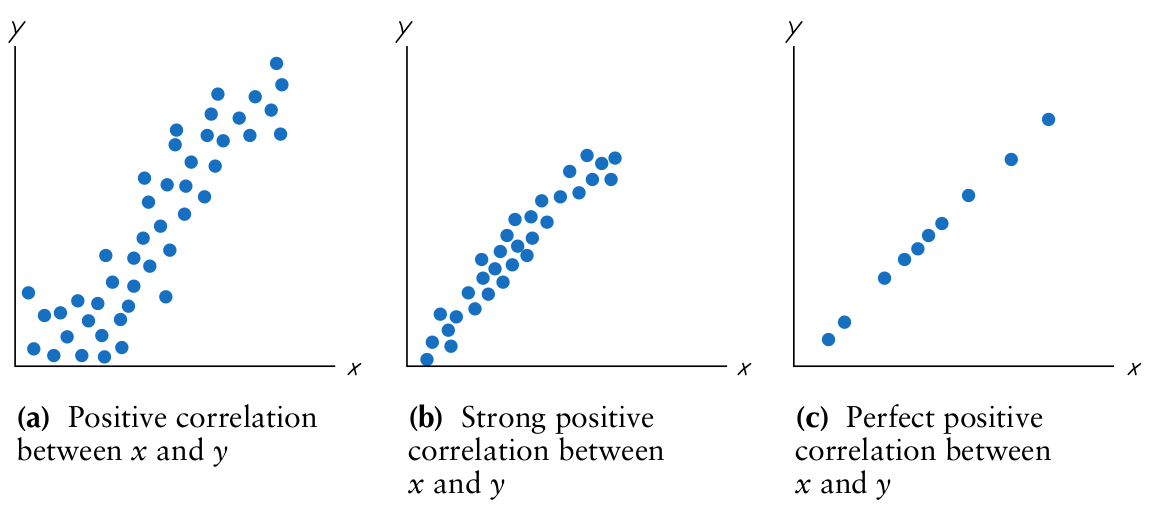
\includegraphics[height=0.6\textheight]{Assoc/positive}

  (Fonte: Triola)
\end{frame}

\begin{frame}{Exemplo}
  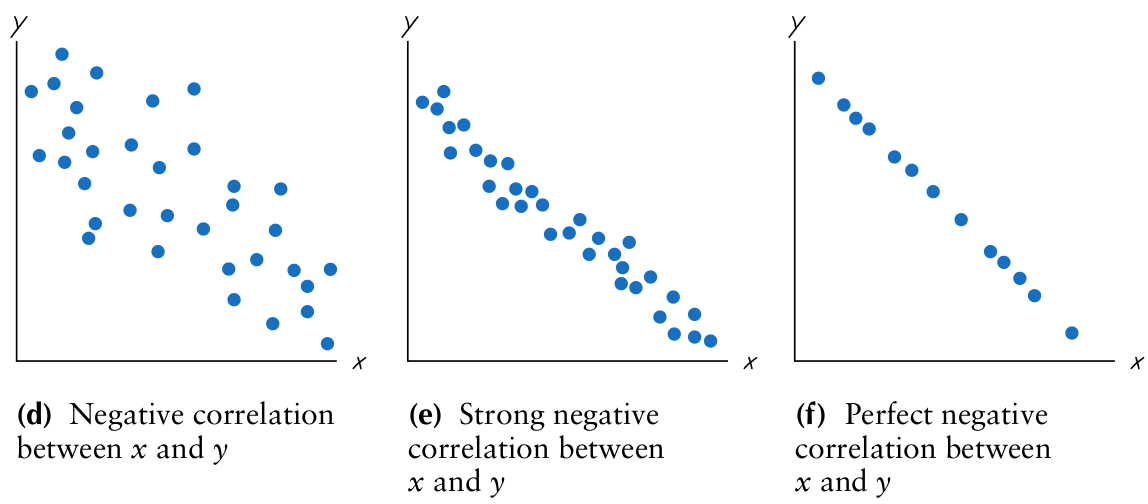
\includegraphics[height=0.6\textheight]{Assoc/negative}

  (Fonte: Triola)
\end{frame}

\begin{frame}{Exemplo}
  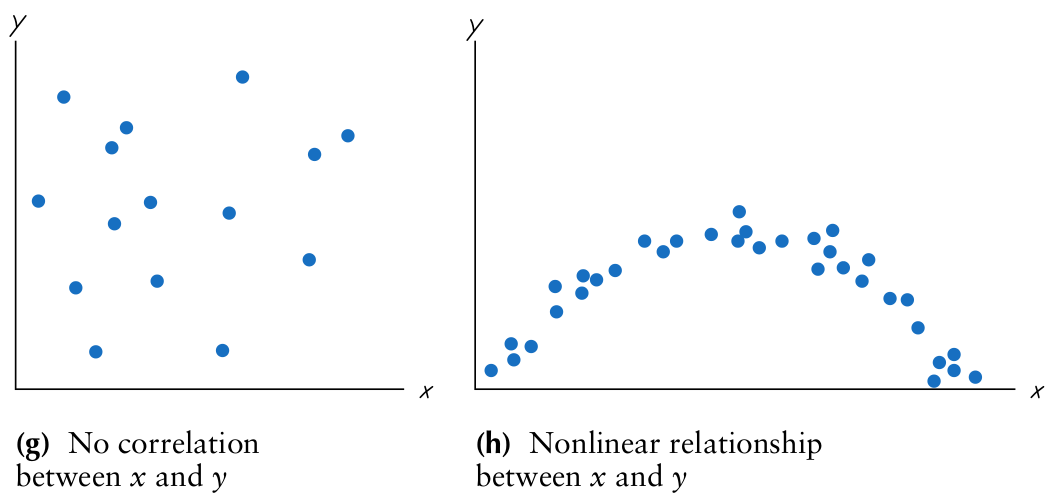
\includegraphics[height=0.6\textheight]{Assoc/other}

  (Fonte: Triola)
\end{frame}

\subsection[Covariância]{Covariância entre duas amostras}

\begin{frame}{Variância}
  \begin{itemize}
  \item Relembrando: a variância (assim como o desvio-padrão) é uma
    medida da dispersão da amostra
  \item Medida sumária que resume o quanto os dados se desviam da
    média
  \item Podemos usar um raciocínio análogo para comparar quanto uma
    amostra se desvia em relação à outra
  % \item Isto é, quanto uma 
  \end{itemize}
\end{frame}

\begin{frame}{Covariância entre duas amostras}
  \begin{definition}
    A covariância entre duas variáveis X e Y é uma medida de quanto
    ambas variam juntas (uma em relação à outra).
  \end{definition}
  \begin{itemize}
  \item Obs: duas variáveis independentes tem covariância igual a zero!
  \end{itemize}
\end{frame}

\begin{frame}{Correlação}
  \begin{definition}
    A correlação é a associação estatística entre duas variáveis.
  \end{definition}
  
  Para medir essa associação, calculamos o \alert{coeficiente de
    correlação} $r$.
  
\end{frame}


% \begin{frame}{}
%   \begin{itemize}
%   \item 
%   \end{itemize}
% \end{frame}

\subsection[Pearson]{Coeficiente de correlação de Pearson}

\begin{frame}{Coeficiente de correlação}
  \begin{definition}
    O coeficiente de correlação $r$ é a medida da direção e força da
    associação entre duas variáveis.
  \end{definition}
  Propriedades:
  \begin{itemize}
  \item É um número entre $-1$ e $1$.
  \item Mede a associação \alert{linear} entre duas variáveis.
    \begin{itemize}
    \item Diretamente proporcional, inversamente proporcional, ou
      ausência de proporcionalidade.
    \end{itemize}
  \end{itemize}
\end{frame}

\begin{frame}{Coeficiente de correlação}
  \begin{itemize}
  \item O coeficiente de correlação de Pearson é a covariância
    normalizada
  \item Pode ser calculado para populações ($\rho$) ou amostras ($r$)
  \item População
    \begin{displaymath}
      \rho = \frac{\text{Cov(X,Y)}}{\sigma_X \sigma_Y}
    \end{displaymath}
  \item Utilizando uma fórmula semelhante, encontramos o coeficiente
    $r$ para uma amostra
  \end{itemize}
\end{frame}

\begin{frame}{Correlação}
  \begin{block}{}
    \begin{itemize}
    \item Uma forte associação \alert<2>{positiva} corresponde a uma correlação
      próxima de \alert<2>{1}.
    \item Uma forte associação \alert<3>{negativa} corresponde a uma correlação
      próxima de \alert<3>{-1}.
    \item A \alert<4>{ausência} de associação corresponde a uma
      correlação próxima de \alert<4>{0}.
    \end{itemize}
  \end{block}
\end{frame}

\begin{frame}{}
  \begin{itemize}
  \item Se tivéssemos os dados de toda a \alert<1>{população}, poderíamos
    calcular o \alert<1>{parâmetro} $\rho$
  \item Na prática, só podemos calcular a \alert<2>{estatística} $r$ da \alert<2>{amostra}
  \item Utilizamos $r$ como estimador para $\rho$, e testamos a
    significância estatística da forma usual
  \end{itemize}
\end{frame}

\begin{frame}{Exemplo}
 \begin{example}
   Pesquisadores queriam entender por que a insulina varia tanto entre
   indivíduos. Imaginaram que a \alert<2>{composição lipídica} das células do
   músculo afetam a \alert<3>{sensibilidade do músculo para a insulina}. Para
   isto, eles injetaram insulina em 13 jovens adultos, e determinaram
   quanta glicose eles precisariam injetar nos sujeitos para manter o
   nível de glicose sanguínea constante. A quantidade de glicose
   injetada para manter o nível sanguíneo constante é, então, uma
   medida da sensibilidade à insulina.

 % Eles só precisavam injetar
   % muita glicose quando o músculo era muito sensível à insulina.

    (Fonte: Motulsky, 1995)
  \end{example}
\end{frame}

\begin{frame}{Exemplo}
  \begin{example}
    Os pesquisadores fizeram uma pequena biópsia nos músculos para
    aferir a fração de ácidos graxos poli-insaturados que tem entre 20
    e 22 carbonos (\%C20-22). Como variável resposta, mediram o índice
    de sensibilidade à insulina.
    % \begin{itemize}
    % \item A variável independente (X) é a quantidade de ácidos graxos
    % \item A variável dependente (Y) é o índice de insulina medido
    % \end{itemize}
  \end{example}
  Valores tabelados a seguir.
\end{frame}

\begin{frame}{Exemplo}
  \begin{center}
      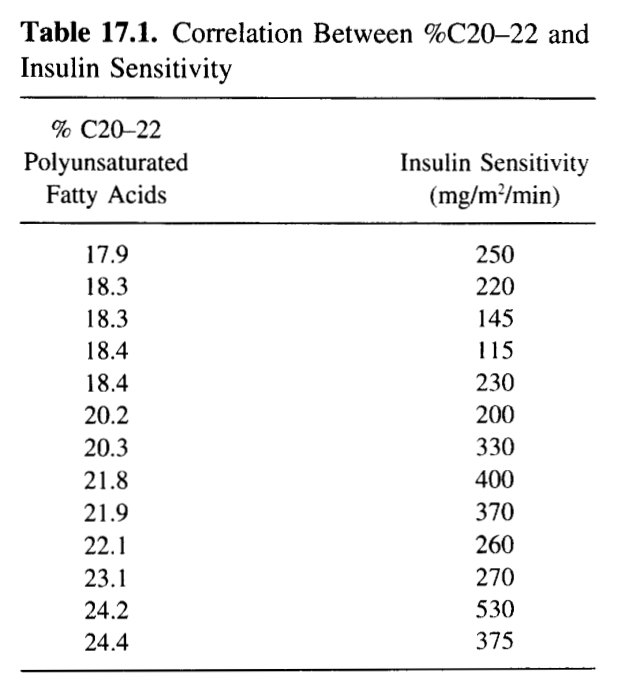
\includegraphics[height=0.8\textheight]{Assoc/table}
  \end{center}
\end{frame}

\begin{frame}{Exemplo: Diagrama de dispersão dos dados}
  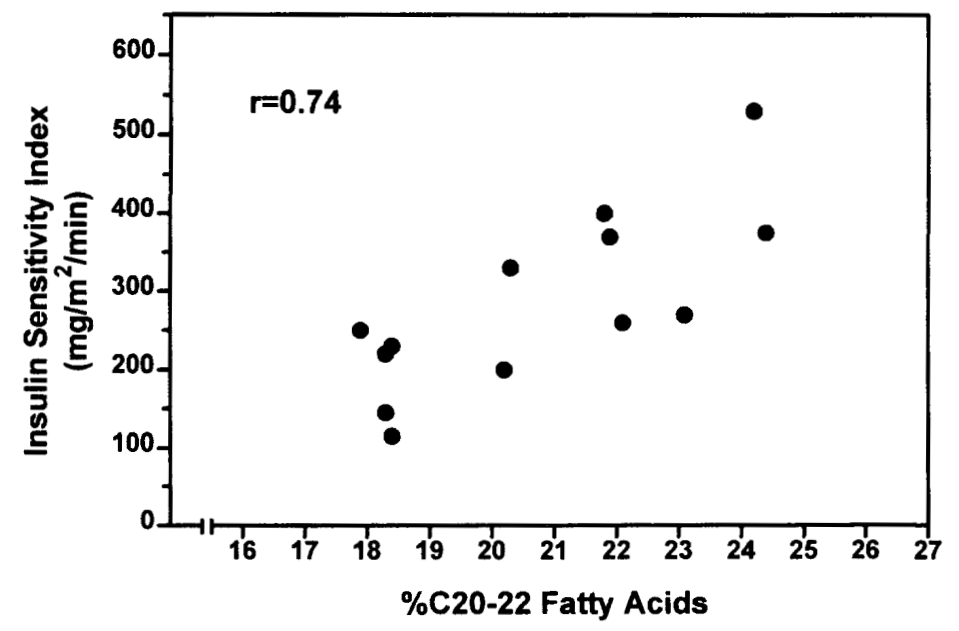
\includegraphics[width=\textwidth]{Assoc/scatter}

  Obs: na verdade, $r=0.77$.
\end{frame}

\begin{frame}{Exemplo}
  \begin{itemize}
  \item O tamanho da amostra foi $n=13$
  \item Consultamos o valor crítico de $r$ na tabela a seguir
  \item Testamos a $H_0$ que não há relação entre as variáveis na
    população ($H_0: \rho = 0$).
  \end{itemize}
\end{frame}

\begin{frame}{Exemplo}
  \begin{center}
      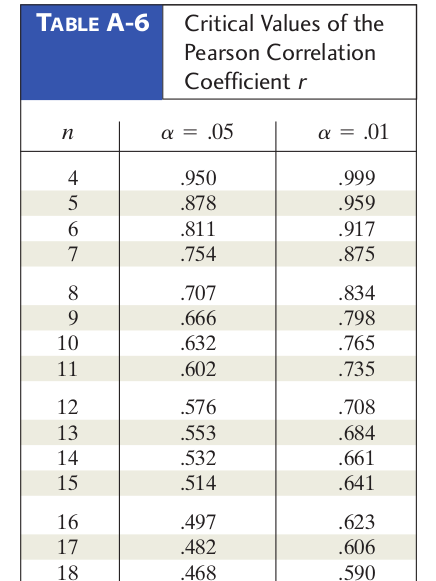
\includegraphics[height=0.8\textheight]{Assoc/test}
  \end{center}
\end{frame}

\begin{frame}{Exemplo}
  \begin{itemize}
  \item O valor crítico da tabela para uma amostra de tamanho 13 é
    $r_c = 0.553$
  \item A correlação calculada para esta amostra foi $r=0.77$
  \item Como a correlação é maior que o valor crítico, a relação é
    estatisticamente significativa
  \item Conclusão: há evidências para rejeitar a $H_0$ que não há
    relação entre as variáveis.
  \end{itemize}
\end{frame}

\begin{frame}{Exemplo}
  \begin{itemize}
  \item Pode-se também calcular o p-valor para o coeficiente de
    correlação $r$.
  \item Para este exemplo, teríamos $p=0.0021$.
  \item Interpretação: se não houver relação entre as variáveis
    ($H_0$), existe apenas 0.21\% de chance de observamos uma
    correlação tão forte com um estudo deste tamanho
  \end{itemize}
\end{frame}

\begin{frame}{Exemplo}
  Por que as duas variáveis são tão correlacionadas? Considere 4
  possibilidades:
  \begin{enumerate}
  \item o conteúdo lipídico das membranas \alert<1>{determina} a
    sensibilidade à insulina
  \item A sensibilidade à insulina de alguma forma afeta o conteúdo lipídico
  \item tanto o conteúdo lipídico quanto a sensibilidade à insulina
    estão sob o efeito de \alert<3>{algum outro} fator (talvez algum hormônio)
  \item as duas variáveis não são correlacionados na população, e a
    estimativa observada nessa amostra é mera coincidência
  \end{enumerate}
\end{frame}

\begin{frame}{Interpretando o $r$}
  \begin{itemize}
  \item Nunca devemos ignorar a última possibilidade (erro tipo I)!
  \item o p-valor indica quão rara é essa coincidência
  \item neste caso, em apenas 0.21\% dos experimentos não haveria uma
    correlação real, e estaríamos cometendo um erro de interpretação
  \end{itemize}
\end{frame}

\begin{frame}{Elevando o $r$ ao quadrado}
  \begin{itemize}
  \item Relembrando: calculamos a variância de uma amostra para saber
    a dispersão dos dados
  \item Sua interpretação é confusa, portanto preferimos usar o
    desvio-padrão
  \item No caso do $r$ é o contrário: a interpretação de $r^2$ é mais simples
  \item Obs: o valor $r^2$ também é chamado \alert{coeficiente de
      determinação}, como veremos a seguir.
  \end{itemize}
\end{frame}

\begin{frame}{Interpretando o $r^2$}
  \begin{itemize}
  \item No exemplo anterior, $r^2 = 0.59$
  \item no caso, 59\% da variabilidade da tolerância à insulina pode
    ser explicada pelo conteúdo lipídico
  \item Ou seja: conhecer o conteúdo lipídico permite explicar 59\%
    da variância na sensibilidade à insulina
  \item Isto deixa 41\% da variância que pode ser explicada por outros
    fatores ou erros de medição
  \item E este valor ($r^2$) também é utilizado na Regressão!
  \end{itemize}
\end{frame}

% \subsection[IC]{Intervalo de Confiança}

% \begin{frame}{Intervalo de confiança em torno de $r$}
%   \begin{itemize}
%   \item 
%   \end{itemize}
%   \begin{example}
    
%   \end{example}
% \end{frame}

% \begin{frame}{Intervalo de confiança em torno de $r^2$}
%   \begin{itemize}
%   \item Com o IC em torno de $r$, podemos obter o IC em torno de $r^2$
%   \item Para isto, basta elevar cada extremo do IC ao quadrado
%   \end{itemize}
%   \begin{example}
    
%   \end{example}
% \end{frame}

\section[Regressão]{Regressão Linear Simples}

\subsection{Modelos estatísticos}

\begin{frame}{Modelos estatísticos}
  Modelos servem para:
  \begin{itemize}
  \item representar de forma simplificada fenômenos, experimentos,
    dados, etc;
  \item possibilitar análise em cenários controlados, menos complexos
    que a realidade;
  \item extrapolar resultados e conclusões.
  \end{itemize}
\end{frame}

\begin{frame}{Modelos estatísticos}
  Ao ajustar um modelo aos dados, podemos:
  \begin{itemize}
  \item fazer predições dentro do intervalo observado para dados que
    não foram obtidos (interpolação)
  \item fazer predições fora do intervalo observado (extrapolação)
  \end{itemize}
\end{frame}

\begin{frame}{Reta de regressão}
  \begin{definition}
    Uma \alert{reta de regressão} (também chamada de reta de melhor
    ajuste) é a reta para a qual a soma dos erros quadráticos dos
    resíduos é o mínimo.
  \end{definition}
  \begin{itemize}
  \item É a reta que melhor se ajusta aos dados
  \item Minimiza os resíduos
  \end{itemize}
\end{frame}

\begin{frame}{Resíduos}
  \begin{center}
      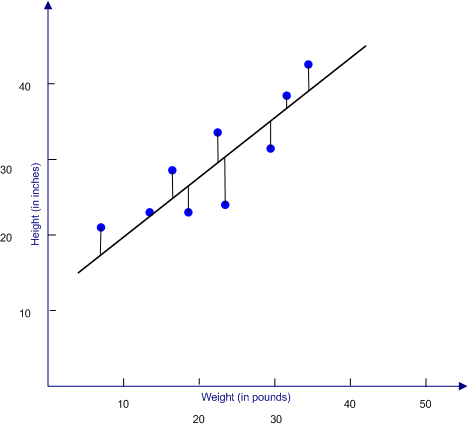
\includegraphics[height=0.6\textheight]{Assoc/residuos}
  \end{center}

  \begin{definition}
    Resíduos são a distância entre o dado observado e a reta estimada
    (modelo).
  \end{definition}
\end{frame}

\begin{frame}{Elementos da reta de regressão}
  \begin{itemize}
  \item Relembrando: a equação de uma reta é definida pela fórmula
    \begin{displaymath}
      \hat{y} = \alert{a} x + \alert{b}
    \end{displaymath}
  \item No caso da reta regressora:
    \begin{itemize}
    \item $y$ é a variável dependente
    \item $x$ é a variável independente
    \item $a$ é a inclinação
    \item $b$ é o intercepto
    \end{itemize}
  \item Assim, o objetivo da análise de regressão é encontrar os
    valores \alert{$a$} e \alert{$b$}
  \end{itemize}
\end{frame}

\begin{frame}{Análise de Regressão}
  Para determinar a inclinação e o intercepto, usamos:
  \begin{itemize}
  \item as médias de $X$ e $Y$
  \item as variâncias de $X$ e $Y$
  \item o coeficiente de correlação $r$ entre $X$ e $Y$
  \item o tamanho da amostra $n$
  \item \ldots e algumas operações entre estes termos
  \end{itemize}
\end{frame}

\subsection{A regressão}

\begin{frame}{Exemplo}
  \begin{example}
    Voltemos ao exemplo de associar a composição lipídica com a sensibilidade a insulina.    
  \end{example}
  \begin{block}{Pergunta}
    Qual é o acréscimo na sensibilidade à insulina, para cada unidade aumentada na composição lipídica?
  \end{block}
\end{frame}

\begin{frame}{Exemplo}
  \centering
  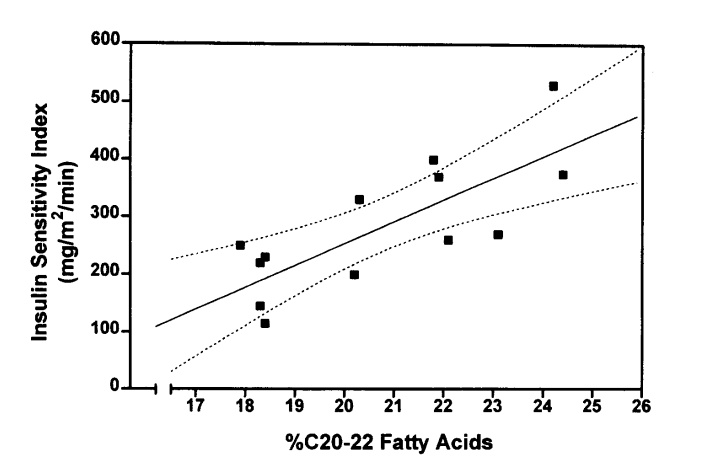
\includegraphics[width=.9\textwidth]{Assoc/regressao1}

  \vfill
  Fonte: Motulsky, 1995
\end{frame}

\begin{frame}{Exemplo}
  \centering
  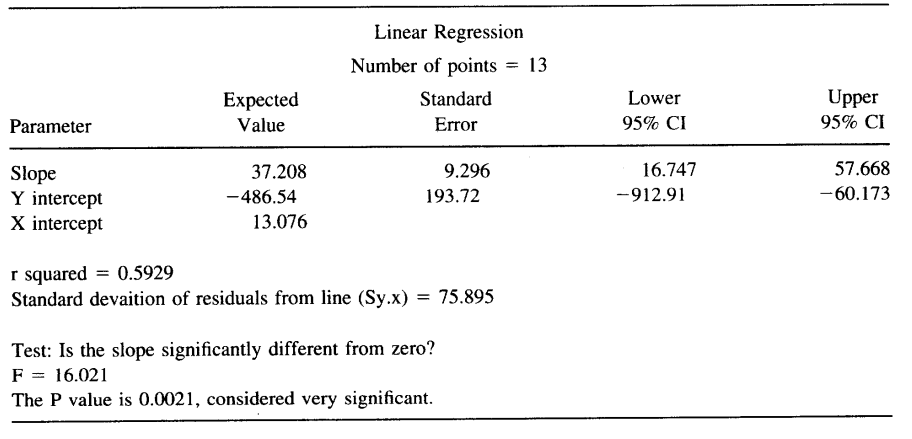
\includegraphics[width=1.2\textwidth]{Assoc/regressao2}
\end{frame}

\begin{frame}{Interpretação}
  \begin{itemize}
  \item O p-valor é significativo.
  \item A inclinação é $\approx \alert{37.2}$
  \item Isto significa que:
  \end{itemize}
  \begin{block}{}
    para cada unidade aumentada no \%C20--22, teremos um aumento proporcional de aproximadamente 37.2 mg/m$^2$/min na sensibilidade à insulina
  \end{block}
\end{frame}

\begin{frame}{Análise de Regressão}
  \begin{center}
      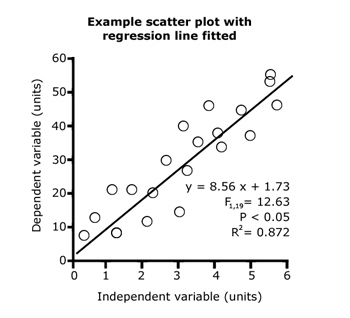
\includegraphics[height=0.6\textheight]{Assoc/residuos2}
  \end{center}

  \begin{itemize}
  \item A qualidade do ajuste do modelo de regressão é determinado
    pelo \alert{coeficiente de determinação} $r^2$
  % \item A semelhança de nomenclatura com o coeficiente $r$ não é mera
  %   coincidência.
  \end{itemize}
\end{frame}

  % Encontrando a inclinação e o intercepto da reta, podemos estimar
  % $\hat{Y}$ para valores arbitrários de $X$.

\subsection[$R^2$]{Coeficiente de Determinação $r^2$}

\begin{frame}{Coeficiente de Determinação $r^2$}
  \begin{definition}
    O \alert{coeficiente de determinação} $r^2$ é a relação da
    variação explicada com a variação total.
  \end{definition}
  \begin{displaymath}
    r^2 = \frac{\text{variação explicada}}{\text{variação total}}
  \end{displaymath}
  \begin{itemize}
  \item Lembrando: $r^2$ é o quadrado de $r$!
  % \item Este valor tem uma interpretação prática mais fácil, que
  %   veremos em breve
  \end{itemize}
\end{frame}

\begin{frame}{Coeficiente de Determinação $r^2$}
  \begin{itemize}
  % \item A variância dos dados pode ser explicada de várias formas
  \item Qual é a porcentagem da variação dos dados pode ser explicada
    pela reta regressora?
  \item O coeficiente $r^2$ é a fração da variância que é
    compartilhada entre $X$ e $Y$.
  \item Como $r$ está sempre entre -1 e 1, $r^2$ está sempre entre 0 e
    1.
  \end{itemize}
\end{frame}

\begin{frame}{Coeficiente de Determinação $r^2$}
  \begin{itemize}
  \item Além disso, $r^2 \le |r|$
  \item Por que?
  \end{itemize}
  \begin{block}{}
    Compare os seguintes números entre 0 e 1:
    \begin{displaymath}
      \frac{1}{2} \text{ e } \left(\frac{1}{2}\right)^2=\frac{1}{4} \Rightarrow
      \frac{1}{4} \le \frac{1}{2}
    \end{displaymath}
    \begin{displaymath}
      \frac{1}{3} \text{ e } \left(\frac{1}{3}\right)^2=\frac{1}{9} \Rightarrow
      \frac{1}{9} \le \frac{1}{3}
    \end{displaymath}
  \end{block}
\end{frame}


% \begin{frame}{Coeficiente de Determinação $r^2$}
%   \begin{itemize}
%   \item 
%   \end{itemize}
% \end{frame}


\section{Interpretação}
% \subsection{Interpretação}

\begin{frame}{Interpretação}
  \begin{itemize}
  \item Se a correlação é 0, então X e Y não variam juntos (independentes)
  \item Se a correlação é positiva, então quando uma aumenta, a outra
    aumenta em proporção direta (linear)
  \item Se a correlação é negativa, então quando uma aumenta, a outra
    diminui em proporção inversa (linear)
  \end{itemize}
\end{frame}


\begin{frame}{Cuidado!}
  \begin{itemize}
  \item Duas variáveis podem \alert{parecer} correlacionadas pois são
    influenciadas por uma terceira variável
  \item Ex: em alguns países a mortalidade infantil é negativamente
    correlacionada com o número de telefones per capita
  \item Mas comprar mais telefones não vai salvar crianças!
  \item Explicação alternativa: a melhoria da condições financeiras
    pode afetar ambas as variáveis
% tanto a quantidade de telefones, quanto a longevidade
    % infantil
  \end{itemize}
\end{frame}

\section{Causalidade}
% \subsection{Causalidade}


\begin{frame}{Causa x efeito}
  \begin{itemize}
  \item Se há uma relação de causalidade entre as duas variáveis, a
    correlação será não nula (positiva ou negativa)
  \item Quanto maior for a relação de dependência entre as variáveis,
    maior será o módulo da correlação.
  \item Se as variáveis não são relacionadas, a correlação será nula.
  \end{itemize}
\end{frame}

\begin{frame}{Causalidade?}
  \begin{itemize}
  \item Mas não podemos inverter a afirmativa lógica do slide
    anterior!
  \item Isto é, ao observar uma forte correlação, gostaríamos de
    concluir que uma variável \alert{causa} este efeito na outra
  \item Infelizmente isto não é possível!
  \item Lembre-se: a significância do teste indica a probabilidade de
    se cometer um erro do tipo I (falso positivo).
  \end{itemize}
  \begin{block}{Repita várias vezes mentalmente}
    Correlação não implica em causalidade.
  \end{block}
\end{frame}

% \begin{frame}{}
%   \begin{itemize}
%   \item 
%   \end{itemize}
% \end{frame}

\begin{frame}{Exemplo}
  Gasto com C\&T (EUA) x Suicídios por enforcamento
  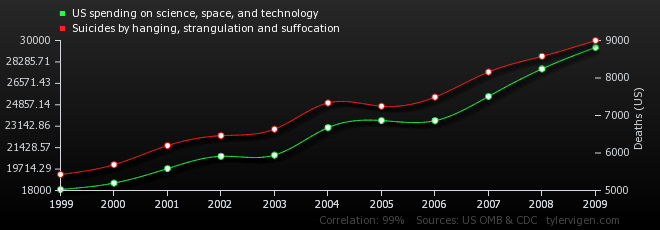
\includegraphics[width=\textwidth]{Assoc/us-spending-on-science-space-and-technology_suicides-by-hanging-strangulation-and-suffocation}

  Correlação: 0.992082

  (Fonte: Spurious correlations)
\end{frame}

\begin{frame}{Exemplo}
  Produção de mel x Prisões por posse de maconha
  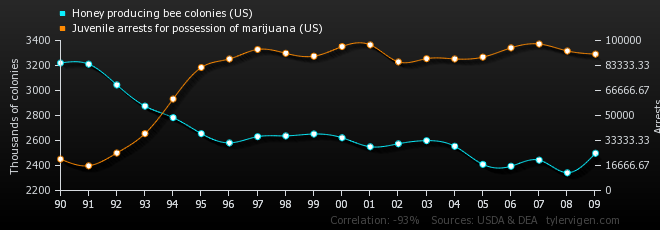
\includegraphics[width=\textwidth]{Assoc/honey-producing-bee-colonies-us_juvenile-arrests-for-possession-of-marijuana-us}

  Correlação: -0.933389

  (Fonte: Spurious correlations)
\end{frame}

\begin{frame}{Exemplo}
  Afogamentos em piscina x Filmes com Nicholas Cage
  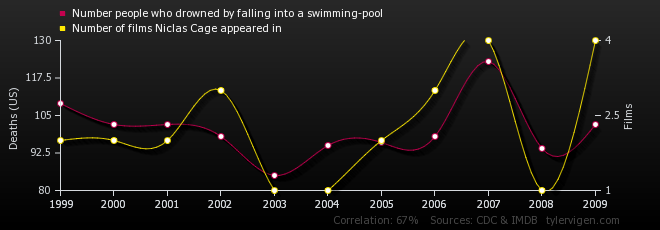
\includegraphics[width=\textwidth]{Assoc/number-people-who-drowned-by-falling-into-a-swimming-pool_number-of-films-niclas-cage-appeared-in}

  Correlação: 0.666004

  (Fonte: Spurious correlations)
\end{frame}

\begin{frame}{Causa e efeito}

  Ao encontrar uma forte correlação, deve-se sempre se perguntar:

  \begin{enumerate}
  \item Há uma relação direta de causa e efeito entre as variáveis? (X
    causa Y?)

  \item Há uma relação inversa de causa e efeito entre as variáveis?
    (Y causa X?)

  \item É possível que a relação entre as variáveis possa ser causada
    por uma terceira variável (ou mais) que não foi analisada?

  \item É possível que a relação entre duas variáveis seja uma
    coincidência?
  \end{enumerate}
\end{frame}

\section{Resumo}
\begin{frame}{Resumo}
  \begin{itemize}
  \item É necessário investigar a relação entre as variáveis!
  \item O que pode explicar a relação observada?
  \item Qual proporção (porcentagem) da variabilidade pode ser
    explicada pelas variáveis analisadas?
  \item Quão bem a reta regressora se ajusta aos dados?
  \end{itemize}
\end{frame}

% \begin{frame}{}
% \end{frame}

\end{document}
